%!TEX root = thesis-kdyoung.tex

\begin{savequote}%[45mm]
---Divide et impera\\
(Divide and conquer)
\qauthor{Philip II of Macedon}
\end{savequote}


\chapter{Benders Decomposition}
\label{chap:benders}
In this chapter we detail the Benders decomposition of the SUALBSP-2. 
The formulation of our logic-based decomposition can be separated into three primary pieces. 
The first is the formulation of the relaxed master problem and the approach used to solve it,
which is detailed in Section \ref{sec:bend:RMP}. 
Similar to the first, we secondly detail our formulation of the sub-problems.
The combinatorial structure that arises in the sub-problems allows multiple possible formulations
and solving procedures, which are overviewed in Section \ref{sec:bend:SP}.
Sections \ref{sec:bend:mipForm}, \ref{sec:bend:cpForm} and \ref{sec:bend:TSP}
each detail a possible approach to formulating
the sub-problems.
% We explain and justify the choices made when modelling the sub-problems.

The last ingredient needed for a full specification of a logic-based Benders decomposition
is how the relaxed master and sub-problems communicate during
the iteration of the algorithm.
As such, we present the Benders cuts which we studied and note each one's
possible strengths and weaknesses depending on the solution procedure.
The Benders cuts we formulated are devised and proven to be valid 
in Section \ref{sec:bend:cuts}.
These cuts, and how they can improve the 
practical effectiveness and efficiency of this approach,
is our primary contribution to the literature.
We close this chapter in Section \ref{sec:bend:alg}, by summarising
the algorithm used to iterate through
the Benders decomposition and our cut-generation scheme.

\section{The Decomposition}
\label{sec:bend:decomp}
We begin this chapter with an overview of how the
\sua{2} can be decomposed.
There are two distinct types of decisions in the problem
and as a result this provides the basis
of our decomposition approach.

% The basis of our decomposition is the MIP formulation
% presented in the previous chapter, \fsbf{2},
% and so there are numerous similarities between
% the decomposition and this model.
We viewed the primary decisions to be the assignment
of tasks to stations and the secondary decisions
as the execution times for each task within a station.
As such, the relaxed master problem is similar to the classical
\sab{2}, where the only concern is allocating the tasks to 
stations.
The assignment found by the master should still
be a precedence-feasible solution, however the setup
times will be relaxed.
As such, the cycle time estimated by the 
RMP will be the maximum load among the stations
with setups assumed to be zero.
% When solving the \sua{2} our objective is to minimize the cycle time
% of the assembly line which closely depends on the
% setup time incurred within each station.
% To prevent the master problem from initially finding unrealistic
% estimates of the cycle time, we could include some
% information about the scheduling problem inside the master.

Once the master problem is solved to optimality,
$m$ sub-problems arise --- one corresponding to each station ---
which take the subset of assigned tasks as input.
The objective of each sub-problem is to find the optimal
schedule of the tasks such that the precedence relations
are respected and the station's workload is minimized.
As mentioned earlier in Chapter \ref{chap:intro},
a sub-problem can be viewed as similar to the asymmetric TSP.
After solving each sub-problem to optimality or detecting infeasibility,
we can pass this information 
back to the master in the form of Benders cuts.	
If a station's minimal possible workload could not respect the
master's relaxed cycle time value, then we need to devise
a Benders cut to reflect this.

In Figure \ref{fig:bend:highLevelBend} we present the framework
of how our Benders decomposition iterates between
the partitions of the problem.
\begin{figure}[tpb]
	\centering
	\caption{Framework of our logic-based Benders decomposition}
	\vspace{2mm}
	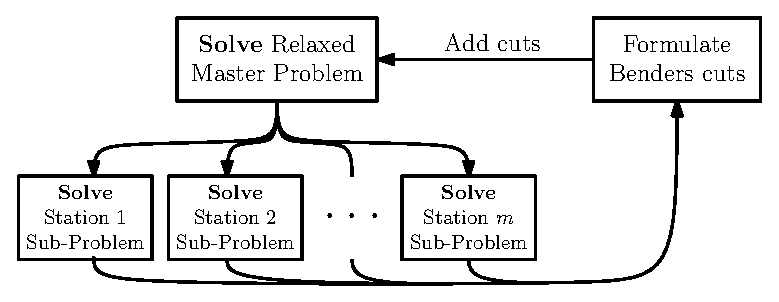
\includegraphics[width=0.9\textwidth]{images/ourHighLevelBenders.eps}
	\label{fig:bend:highLevelBend}
\end{figure}

\section{Types of Sub-Problems}
\label{sec:bend:SPtype}
When using logic-based Benders decomposition, there are two general types 
of sub-problems which can be implemented: optimality sub-problems and 
feasibility sub-problems.
We now detail the unique qualities of each 
type and discuss their possible advantages and disadvantages when 
applied to the \sua{2}.

\subsection{Feasibility Sub-Problems}
\label{sec:bend:SPfeas}
Using feasibility sub-problems means that we are only required to check if 
the relaxed master's current solution is feasible.
If the sub-problems are found to be infeasible given the master's cycle time, 
then a cut-set is sent back to the master to remove
this assignment and similar assignments from the master's feasible solution space.
Testing for infeasibility can be a fast procedure as only
one sub-problem needs to report that its assignment cannot
satisfy the master's cycle time.
Although the trade-off here is that feasibility sub-problems
provide a comparatively small amount of information when compared to optimality sub-problems.
This could mean that the speed we gain from only testing for
feasibility could be dwarfed by the reduction in cut quality.
In fact, low quality Benders cuts can lead to more iterations of
the algorithm being required; if the primary bottleneck in computational runtime
is due to the master then simpler sub-problems may not
provide an overall runtime reduction.
Even so, it is not necessarily the case that feasibility sub-problems 
are strictly worse than optimality sub-problems.

In the case of the \sua{2} we have $m$ sub-problems at 
each iteration of the decomposition. 
If we consider feasibility sub-problems, then there are two simple 
but quite distinct ways which the cutting procedure could 
possibly be formulated. 
% We detail these here and what is gained and lost with each formulation.
\begin{itemize}
	\item \emph{Solve all sub-problems}. By testing the feasibility of each station's
	assignment, we find out all stations which are infeasible
	and all which can satisfy the cycle time.
	This allows $k$ Benders cuts to be made where $k$ is the number
	of sub-problems where infeasibility is detected ($k \leq m$).
	Each sub-problem can be run in parallel which can vastly reduce the solution
	time of the sub-problems, however parallel computation isn't strictly necessary
	in this case.
	\item \emph{Solve until infeasibility}. Run all sub-problems in parallel until
	one detects infeasibility, then terminate all other problems.
	This procedure will be much faster than the last however we gain far less information
	from the sub-problems.
	In this case we can make only two Benders cuts.
	The sub-problem which found infeasibility results in a Benders cut
	that removes its assignment of tasks from the master's feasible region.
	We can also make a weaker cut that removes the
	full assignment of tasks from occurring in future
	iterations.
\end{itemize} 

In both cases of feasibility sub-problems, the information
gained is limited and so the range of Benders cuts we can formulate
is quite restricted.
The feasibility cuts we considered are presented later in Section \ref{sec:bend:NGcuts}.

\subsection{Optimality Sub-Problems}
\label{sec:bend:SPopt}
Programming the scheduling problem within each
station as an optimality sub-problem means that
the optimal sequence of tasks within each station
will be found; irrelevant of whether a station's
load can respect the master's cycle time estimate.
The disadvantage of this when compared to
just testing for infeasibility, is that
solving each combinatorial scheduling problem
to optimality may be far more time consuming.
The primary advantage is that at each iteration
of the Benders algorithm, we receive richer information
from the sub-problems allowing more flexibility in
the Benders cuts we devise.

% Unlike feasibility sub-problems, there is little computational speed we can gain
% by taking advantage of parallel computing here.
% Running all sub-problems in parallel could certainly
% result in a reduction in total runtime, but as each
% scheduling problem needs to be solved to optimality, there is no more
% we can gain via the communication of solutions between sub-problems.

We predominantly explored the use of optimality cuts in our
Benders decomposition and in the coming sections 
(see \ref{sec:bend:Icuts1}--\ref{sec:bend:Logcuts}) we will
provide their formulation.

\section{Relaxed Master Problem}
\label{sec:bend:RMP}
The relaxed master problem handles the assignment
of tasks to stations.
As mixed-integer programming is an effective solving technology for
allocation problems (refer to Section \ref{sec:lit:hybridBend})
we formulated the RMP as a MIP.

Let the current iteration of the Benders
algorithm be indexed by $\mu$
and a previous iteration by $\nu$.
We now present the formulation of the RMP 
at the $\mu^{th}$ iteration, which we will denote
by \rmp{\mu}.
% The decision variables of this program are summarised
% in Table \ref{tab:bend:RMPvars}.
The cycle time variable, $c^\mu$, and the assignment
variables, $x_{ik}^\mu$, have equivalent definitions
as in the previous chapter but are now also indexed by the 
Benders iteration counter.
% Variables $y_{ijk}$ and $z_{ijk}$ allow the master to decide
% upon a sequencing of the tasks within each station
% and these variables are defined equivalently as in the previous
% chapter.
The complications presented by the sequencing problems
are omitted from the RMP and as a result the total setup
cost of each station is taken as zero.
% The estimated setup cost of station $k$ is decided by
% variable $\xi_k$.

\begin{IEEEeqnarray}{rClCl}
	\IEEEeqnarraymulticol{3}{l}{\text{\rmp{\mu}: Min } c^\mu} & \hspace{4mm} & \label{eq:bend:rmp1}\\[\eqnv]
	\text{s.t. } & \hspace{4mm} & \sum_{k\in FS_i} x_{ik}^\mu = 1 & & \forall i \in V \label{eq:bend:rmp2}\\[\eqnv]
	& & \sum_{k \in FS_i} k\cdot x_{ik}^\mu \leq \sum_{k \in FS_j} k\cdot x_{jk}^\mu & & \forall (i,j) \in E \label{eq:bend:rmp3}\\[\eqnv]
	& & \sum_{i \in V} t_i \cdot x_{ik}^\mu \leq c^\mu & & \forall k \in K \label{eq:bend:rmp4}\\[\eqnv]
	& & \mathcal{C}^\nu & & \nu \in \{1, 2,\ldots,\mu-1 \} \label{eq:bend:rmp5}\\[\eqnv]
	& & \ul{c}^\mu\leq c^\mu \leq \bar{c}^\mu & &  \label{eq:bend:rmp6}\\[\eqnv]
	& & x_{ik}^\mu\in\{0,1\} & & \forall i \in V,~ k \in FS_i \label{eq:bend:rmp7}
\end{IEEEeqnarray}

The objective is to minimize the cycle time estimate in (\ref{eq:bend:rmp1}).
Constraint (\ref{eq:bend:rmp2}) ensures each task
is assigned exactly one station.
We ensure the precedence relations are satisfied between stations with
constraint (\ref{eq:bend:rmp3}).
Each station's total workload, \ie sum of task processing times,
is required to respect the cycle time through constraint (\ref{eq:bend:rmp4}).
Finally, the set of Benders cuts found in the previous iterations are included
in the master in constraint (\ref{eq:bend:rmp5}).
The remaining constraints define the domains of
each decision variable.

We note here that unlike the MIP formulations presented in the
previous chapter, this relaxed formulation of just the
assignment portion has not required any disjunctive constraints.
Hence, the linear relaxation used throughout the \bab algorithm
of the Gurobi solver will likely be far tighter.

% The RMP is in fact very close to a full formulation
% of the \sua{2}, with only a single requirement removed.
% This is the constraint that within each station we require only a single
% cyclic sequence of tasks.
% So we can view a solution to the RMP as an assignment

\section{Sub-Problems}
\label{sec:bend:SP}
Each of the sub-problems has a similar structure to
the asymmetric Travelling Salesperson Problem
with some forbidden paths.
We can view the tasks as the cities and distance
between any pair of tasks as the setup time.
The asymmetry is due to $\phi_{ij}$ ($\beta_{ij}$) not necessarily
being equal to $\phi_{ji}$ ($\beta_{ji}$).

As the structure of each scheduling problem has a 
highly combinatorial nature we consider 
three approaches:
mixed-integer programming, constraint
programming and fully formulating
the sub-problem as a TSP.
When the sub-problem is formulated
as a constraint program or a TSP,
then the logic-based Benders decomposition
we propose can be seen as a hybrid solution
methodology.

We now define new notation for formulating a
sub-problem.
The set of tasks assigned to station $k$
at iteration $\mu$ is defined as $V_k^\mu \subseteq V$.
The set of precedence relations is given by 
\[
	E_k^\mu = \{\: (i,j) \: | \: i,j \in V_k^\mu\:\} \subseteq E,
\]
The decision variables $y_{ij}$, $z_{ij}$ and $s_{i}$
all have equivalent definitions as in the previous chapter.
The total workload of a station is decided by the variable
$l_k^\mu$.
Table \ref{tab:bend:SPvars} provides a summary of a sub-problem's
decision variables.

\begin{table}[tbp]
	\def\arraystretch{1.1}
	\centering
	\caption{Decision variables of sub-problem $k$ at iteration $\mu$}
	\vspace{2mm}
	\begin{tabular}{lp{0.8\textwidth}}
		\toprule
		Variable & Definition \\\midrule\midrule
		$l_k^\mu$ & Total load of the current station $k$ at iteration $\mu$, $k$ is a parameter for a given sub-problem \\
		$s_i$ & start time of task $i\in V_k^\mu$, continuous \\
		$y_{ij}$ & 1 iff task $i \in V_k^\mu$ is followed directly by task $j \in F_i^\phi$ in the forward station load \\
		$z_{ij}$ & 1 iff task $i \in V_k^\mu$ is the last task completed and task $j \in F_i^\beta$ is the first in the same station \\
		\bottomrule
	\end{tabular}
	\label{tab:bend:SPvars}
\end{table}

\subsection{MIP Sub-Problem Formulation}
\label{sec:bend:mipForm}
Let \spmip{\mu} denote the mixed-integer programming
formulation of the sub-problem at iteration $\mu$.
Given the set $V_k^\mu$ of tasks that need to be sequenced,
we can formulate the MIP as follows

\begin{IEEEeqnarray}{rClCl}
	\IEEEeqnarraymulticol{3}{l}{\text{\spmip{\mu}: Min } l_k^\mu} & \hspace{4mm} & \label{eq:bend:spmip1}\\[\eqnv]
	\text{s.t. } & \hspace{4mm} & \sum_{j \in F_i^\phi} y_{ij} + \sum_{j \in F_i^\beta} z_{ij} = 1 & & \forall i \in V_k^\mu \label{eq:bend:spmip2}\\[\eqnv]
	& & \sum_{i \in P_j^\phi} y_{ij} + \sum_{i \in P_j^\beta} z_{ij} = 1 & & \forall j \in V_k^\mu \label{eq:bend:spmip3}\\[\eqnv]
	& & \sum_{i\in V_k^\mu} \sum_{j\in F_i^\beta} z_{ij} =1 & &  \label{eq:bend:spmip4}\\[\eqnv]
	& & s_i + t_i + \phi_{ij}\cdot y_{ij} \leq s_j & & \forall (i,j) \in E_k^\mu \label{eq:bend:spmip5}\\[\eqnv]
	& & s_i + t_i + \phi_{ij} \leq s_j + M(1-y_{ij}) & & \forall i\in V_k^\mu,~ j \in F_i^\phi  \label{eq:bend:spmip6}\\[\eqnv]
	& & s_i + t_i + \sum_{j\in F_i^\beta}\beta_{ij}\cdot z_{ij} \leq l_k^\mu & & \forall i\in V_k^\mu \label{eq:bend:spmip7}\\[\eqnv]
	& & l_k^\mu \geq 0 & &  \label{eq:bend:spmip8}\\[\eqnv]
	& & s_i \geq 0 & & \forall i \in V_k^\mu \label{eq:bend:spmip9}\\[\eqnv]
	& & y_{ij}^\mu\in\{0,1\} & & \forall i \in V_k^\mu,~ j \in F_i^\phi \label{eq:bend:spmip10}\\[\eqnv]
	& & z_{ij}^\mu\in\{0,1\} & & \forall i \in V_k^\mu,~ j \in F_i^\beta \label{eq:bend:spmip11}
\end{IEEEeqnarray}

Together constraints (\ref{eq:bend:spmip2}) and (\ref{eq:bend:spmip3})
ensure that each task in the station's cyclic sequence
has exactly one successor and one predecessor respectively.
Only one backward setup cost exists in the sequence due
to (\ref{eq:bend:spmip4}) and
the precedence relations are enforced by (\ref{eq:bend:spmip5}).
The disjunctive constraint (\ref{eq:bend:spmip6}) requires
that if tasks $j$ directly follows task $i$ in the sequence,
then the setup cost is observed.
Finally, constraint (\ref{eq:bend:spmip7}) bounds the total station
load below by the completion time of the last task in the station.

Decomposing the full MIP formulation into the assignment and scheduling
components has significantly reduced the number of disjunctive constraints
required. Although, to correctly encode the forward setup time
we still require one disjunctive constraint in \spmip{}.

\subsection{CP Sub-Problem Formulation}
\label{sec:bend:cpForm}
Let \spcp{\mu} denote the CP
formulation of the sub-problem at iteration $\mu$.
We considered a constraint programming formulation
of the sub-problem as CP
is a powerful solution technology available
for scheduling problems (see Section \ref{sec:lit:cp}).

Here we will detail the CP model we formulated
and the various advantages that this approach
provides.
Note, that we will give simplified
snippets of the MiniZinc code of our
CP model.

\subsubsection{Basic CP Model}
\label{sec:bend:cpModel}
The majority of the CP model is very similar
to the MIP.
To give the reader an idea of how a constraint
from a MIP can instead be represented in a constraint program,
we now provide the MiniZinc code which equivalently
encapsulates linear constraint (\ref{eq:bend:spmip2}).
\begin{lstlisting}[language=minizinc]
constraint forall ( i in TASK ) (
      sum( j in followForward[i]  )( y[i,j] )
    + sum( j in followBackward[i] )( z[i,j] ) == 1
);
\end{lstlisting}%\vspace{5mm}
The set {\tt TASK} is equivalent to $V_k^\mu$ in the MIP,
while {\tt followForward[i]} and \newline{\tt followBackward[i]} correspond to
$F_i^\phi$ and $F_i^\beta$ respectively.

All other constraints from the MIP translate in similar ways and
for brevity we will only note the main differences between the
two models.
For the full specification of the CP program, 
we refer the reader to the MiniZinc code included
in the Appendices \ref{lst:appen:CPmodel}.
The expressive nature of CP allows us to more effectively
encode the disjunctive constraint from (\ref{eq:bend:spmip6}).
This can be done as follows,
\begin{lstlisting}[language=minizinc]
constraint forall ( i in TASK, j in followForward[i] ) (
    y[i,j] <-> ( s[i] + dur[i] + forwardSetup[i,j] == s[j] )
);
\end{lstlisting}%\vspace{5mm}
Where {\tt dur[i]} corresponds to $t_i$ and {\tt forwardSetup}
stores the two-dimensional array of forward setup times, $\phi_{ij}$.
Using the bijection operator, {\tt <->}, offered by MiniZinc,
we are able to succinctly create two conditional constraints
in the constraint model.
Also, notice that previously this constraint was encoded
as an inequality, however now we are able to fix the starting
time of task $j$ if we know that task $i$ is its direct predecessor.
The flexibility and expressiveness of the CP language MiniZinc
has allowed us to remove many of the negative qualities of this disjunctive
constraint.

\subsubsection{Global Scheduling Constraints}
\label{sec:bend:cpGlob}
Many scheduling problems have been effectively solved
by CP due to the powerful propagation qualities
of the global constraints.
We will now briefly detail some of the global constraints
that are well-suited to our problem
and how they can be utilized.
Note that the constraints presented here
have been somewhat simplified and some of their
more complex functionality is not regarded.

Since within each station no two tasks can be executed
concurrently, the \newline\disj constraint can model this non-overlap property.
This global constraint takes as input two arrays related to a
task: variable start times, 
and fixed durations.
\begin{lstlisting}[language=minizinc]
disjunctive( array of var int: start,
             array of int: dur );
\end{lstlisting}%\vspace{5mm}
In our problem we have start time variables $s_i$
and fixed processing durations $t_i$ for each task,
which suggests \disj could be suited to a sub-problem.
However, the actual duration between any two tasks
$i$ and $j$ is not just the processing time of task $i$,
but also the setup cost $\phi_{ij}$.
Since this setup cost depends on the task ordering, the
duration cannot be fixed.
As such, \disj may not provide as effective propagation
as another global constraint.

The global constraint \cumu ~--- previously described
in Section \ref{sec:lit:cpGlob} ---
is similar to \disj but requires two further
pieces of input: the quantity of resources that each task
requires and also the limit of total available resources.
\begin{lstlisting}[language=minizinc]
cumulative( array of var int: start, 
            array of int: dur, 
            array of var int: resourceRequirement, 
            int: resourceLimit );
\end{lstlisting}%\vspace{5mm}
In our case only one task can be processed within
a station, so we define the resource limit to be 1.
To overcome the problem encountered with the \disj constraint
we introduce a new set of decision variables that are added to
\spcp{}. For each pair of tasks in $V_k^\mu$ we add the continuous variable $\sigma_{ij}$ defined as follows
\[
	\sigma_{ij} =\displaystyle
	\begin{cases}
	s_i &\text{if } y_{ij}=1,\\
	0 &\text{otherwise}.
	\end{cases}
\]
Now that we have a variable defining the start time
of a task $i$ which also depends on task $i$'s place
in the sequence, we can use the \cumu constraint to more accurately
encode the non-overlapping quality of the tasks.
\begin{lstlisting}[language=minizinc]
constraint cumulative(
    [ sigma[i,j]                 | i in TASK, j in TASK ],
    [ dur[i] + forwardSetup[i,j] | i in TASK, j in TASK ],
    [ y[i,j]                     | i in TASK, j in TASK ],
    1
);
\end{lstlisting}%\vspace{5mm}
The start time variables given to cumulative
are the $\sigma_{ij}$ variables.
This requires the \cumu constraint to handle the scheduling of
$n^2$ variables rather than just $n$.
But we hope that
the intelligent propagation it will provide
will outweigh the cost.
Each $\sigma_{ij}$ variable has only a single
corresponding $\phi_{ij}$ and so the durations
sent to \cumu are now fixed values.
Notably, the resource requirement of each task has been
given to the constraint as the variable $y_{ij}$.
So if task $j$ does not directly follow task $i$ in the
task sequence then $y_{ij}$ will take value 0 and the
resource requirement of the corresponding
task in the \cumu constraint will also be 0, \ie
it will not be considered in the schedule.

By achieving an encoding of the non-overlapping quality
between the tasks of a station using a global constraint,
we have allowed the CP sub-problems to gain access
to the well-studied propagation properties of \cumu.

% \subsubsection{Redundant Constraints}
% \label{sec:bend:cpRedun}
% One of the quirks or the MiniZinc language
% is that no decision variable can be defined
% on a non-contiguous set.
% Although, we need the variables $y_{i,j}$
% to be defined $\forall i\in V$ and $\forall j\in F_i^\phi$.
% However $F_i^\phi$ is not necessarily a 
% contiguous set of tasks and so we
% instead defined the $j$
% index over all tasks, \ie $\forall i\in V,~j\in V$.
% Similarly for the $z_{ij}$ variables and the 
% set $F_i^\beta$.
% Consider the following two constraints:
% \begin{lstlisting}[language=minizinc]
% constraint forall ( i in TASK, j in TASK
%                     where not( j in followForward[i] ) ) (
%     y[i,j] == 0
% );
% constraint forall ( i in TASK, j in TASK
%                     where not( j in followBackward[i] ) ) (
%     z[i,j] == 0
% );
% \end{lstlisting}%\vspace{5mm}
% These constraints fix the values of the 
% decision variables $y_{ij}$
% and $z_{ij}$ whose values are known \ap.
% Including these constraints, reduces the 
% amount for work necessary for the solver.

\subsubsection{Search Procedure}
\label{sec:bend:cpSearch}
MiniZinc provides a search language containing
a range of basic search procedures, 
such as \intser and \bolser,
as well as a compositional search procedure,
\seqser, which allows the user to define
problem-specific search strategies.
This allows the user utilize their
familiarity with the problem to direct the 
search tree of the CP solver toward areas
which will likely provide good feasible
solutions.
We note here that including the auxiliary 
variable $\sigma_{ij}$ in the CP model
allowed us to formulate a wider range of
potential search strategies.

We considered a range of basic and compositional
search procedures.
A simplified representation of
the basic procedures are as follows
\begin{lstlisting}[language=minizinc]
ann: start_io = int_search( s, input_order,      indomain_min );
ann: start_sm = int_search( s, smallest,         indomain_min );
ann: start_sl = int_search( s, smallest_largest, indomain_min );  
ann: start_ff = int_search( s, first_fail,       indomain_min ); 

ann: sigma_ff = int_search( [ sigma[i,j] | i in TASK, j in TASK ],
                                first_fail, indomain_max );
\end{lstlisting}%\vspace{5mm}

To briefly illustrate how these procedures
operate, we consider the {\tt start\_sm} search.
In this case, the CP solver will choose to branch on the
start time variables of the tasks first.
The first start time variable that will be chosen, say $s_i$,
will be the one with the smallest value in its domain;
governed by the {\tt smallest} variable selection.
Once chosen, two new nodes will be created:
one with the value of $s_i$ fixed to its smallest
value, and one where this smallest value is removed from
$s_i$'s domain.

We compose these five search annotations in a number of ways using
the \newline{\tt seq\_search} procedure as follows
\begin{lstlisting}[language=minizinc]
ann: start_io_Then_sigma = seq_search([ start_io, sigma_ff ]);
ann: start_sm_Then_sigma = seq_search([ start_sm, sigma_ff ]);
ann: start_sl_Then_sigma = seq_search([ start_sl, sigma_ff ]);
ann: start_ff_Then_sigma = seq_search([ start_ff, sigma_ff ]);
\end{lstlisting}%\vspace{5mm}
Take for example, {\tt start\_sm\_Then\_sigma}.
In this case the start time variables $s_i$ are fully decided
before moving to the $\sigma_{ij}$ variables.
Although having a full solution to $s_i$ will necessarily 
fix all values the $\sigma_{ij}$ variables, since
the full sequence of tasks has been found.
Hence, the compositional procedure has in fact provided
little benefit for us here.

In our computational experiments we compare the
results of some of these basic and compositional
procedures.
Further to this, we compare these results
against the default search of the CP solver
\chuffed to check whether guiding the
branching of the search tree provides a benefit
for this problem.

\subsubsection{Priority Search}
\label{sec:bend:cpPriSearch}
A recent advancement to the search
functionality of MiniZinc by \authciteb{Young2017b}
has provided a new search combinator:
\priser.
We give a brief summary of this compositional
procedure and detail how we have used it
to formulate new search strategies.

The \priser procedure is defined as
\begin{lstlisting}[language=minizinc]
ann: priority_search( ann, ann, array[int] of ann )
\end{lstlisting}%\vspace{5mm}
where the first and second input annotations
can be defined as \emph{selvars} (selection variables)
and \emph{varsel} (selection criteria).
Similar to the sequential search combinator, this search
takes as input an array of other search procedures.
However the extra functionality that \priser
offers is the ability to dynamically change how
the array of search annotation inputs are ordered.
This is unlike the \seqser procedure which required
a fixed list that could not be changed as the search
progressed.
\priser offers the user more flexibility than was previously
available due to the ability to nest priority search strategies.

Here we provide one example of a \priser
that we considered and detail how three other similar
priority search strategies can be formulated.
\begin{lstlisting}[caption={Priority search used for CP sub-problems},label={lst:bend:priser},language=minizinc]
ann: priority_ff = priority_search( s, first_fail,
    [seq_search([
                int_search([ s[i] ],                   first_fail, indomain_min)
                int_search([ sigma[i,j] | j in TASK ], first_fail, indomain_min) ])
    | i in TASK ]
);
\end{lstlisting}\vspace{5mm}
This search is also formulated in three similar ways by
using the {\tt input\_order}, {\tt smallest} and {\tt smallest\_largest}
variable selection strategies instead of {\tt first\_fail}.

As noted earlier, the compositional search
procedure we considered gained little upon the basic
searches they combined.
The priority search, given in Listing \ref{lst:bend:priser},
branches first on the start time of the task
with the fewest possible values in its domain, say task $i$. 
% because of variable selection strategy {\tt first\_fail}.
Once $s_i$ is fixed, we then search over the
start times of variables that can follow task $i$,
\ie the variables $\sigma_{ij}$.
Priority Search allows us to quickly remove
possible followers from consideration and guide the
branching of the search procedure.


\subsection{TSP Sub-Problem Formulation}
\label{sec:bend:TSP}
Let \sptsp{\mu} denote the TSP
formulation of the sub-problem at iteration $\mu$.
Since the sequencing problem within each station is similar to the 
asymmetric version of the TSP, we assumed that
employing a dedicated TSP solver, such as Concorde \cite{Applegate2017},
would be a desirable approach to the sub-problems.

The TSP solver Concorde has been shown to be exceptionally
effective at tackling the symmetric case of the TSP;
solving instances of up to 85,900 cities.
Although the input to the solver is restricted to just 
the symmetric version, if we are able to represent a
station's sub-problem as a symmetric TSP then the computational
runtime reduction may be worthwhile.

Converting an asymmetric TSP to a symmetric version is a straightforward
procedure that results in the number of cities being doubled.
So overcoming that obstacle is possible, however the differentiation
between forward and backward setup times poses another
problem.
This difference means that the city where the travelling salesperson
begins and the final city they visit has an impact on the total tour
length (due to the backward setup).
This complication results in a sub-problem
being distinctly different (but closely related) 
to the TSP.
This difference proved difficult to overcome early in our
exploration of this formulation.
As a result, we focused our attention on the other
possible sub-problems and did not pursue
a TSP formulation further.
However, we do encourage the enthusiastic reader to try their hand 
at such a formulation.

\section{Cuts}
\label{sec:bend:cuts}
The quality of the Benders cuts formulated from the solution
of the sub-problems directly impact the
speed with which the Benders decomposition will
approach the optimal solution.
As such, we considered a range of cuts which
can be added to the master problem, after
all sub-problems have been resolved.
% One type of feasibility cut was devised and is presented in
% Section \ref{sec:bend:NGcuts}.
% The remaining cuts are all instances of optimality
% cuts and are given in Sections \ref{sec:bend:Icuts1}--\ref{sec:bend:Logcuts}.

For this section we introduce new notation detailed
in Table \ref{tab:bend:notationProofs}.
Using this notation we represent a solution to the master 
by its assignment and cycle time
variables as $S^{\nu}=\{[x_{ik}^\nu],c^\nu\}$,
and the optimal solution is represented as
$S^{\nu*}=\{[x_{ik}^{\nu*}],c^{\nu*}\}$.
\begin{table}[tbp]
	\def\arraystretch{1.1}
	\centering
	\caption{Notation for proofs}
	\vspace{2mm}
	\begin{tabular}{lp{0.8\textwidth}}
		\toprule
		Notation & Definition  \\\midrule\midrule
		$\mathcal{C}^\nu$ & The set of all cuts added to the RMP at iteration $\nu$ of the Benders algorithm\\
		$\mathcal{C}_x^\nu$ & The set of type-$x$ cuts added to the RMP at iteration $\nu$, where \newline $x\in\{\:ng,\:i,\:ii,\:iii,\:ub,\:l\:\}$, \eg $\mathcal{C}_{ng}^\nu$ denotes the set of nogood cuts\\
		$\mathcal{F}^\nu$ & The feasible solution space of \rmp{\nu}\\
		$S^\nu ~(S^{\nu*})$ & A feasible (optimal) solution to \rmp{\nu}, $S^\nu\in \mathcal{F}^\nu$\\
		$[x_{ik}^\nu]~ \big( [x_{ik}^{\nu*}] \big)$ & A feasible (optimal) solution to the assignment decisions of \rmp{\nu} \\
		\bottomrule
	\end{tabular}
	\label{tab:bend:notationProofs}
\end{table}

\subsection{Nogood Cut}
\label{sec:bend:NGcuts}
A \emph{nogood} is a partial solution to a problem which prevents
a full feasible solution from being obtained.
In our case, we considered a partial solution to the full problem
to be an assignment of tasks to a single station.
If we consider sub-problem $k$ at iteration $\nu$
then when $l_k^\nu \not\leq c^\nu$ a nogood cut
can be added to the master problem to remove this
partial solution from the feasible solution
space of \rmp{\mu}, where $\mu=\nu+1,\:\nu+2,\:\ldots$.

We now present the formulation of the nogood cut
added to the \rmp{} at iteration $\nu$
and considered for all iterations $\mu>\nu$.
\begin{IEEEeqnarray}{rCcCl}
	\mathcal{C}_{ng}^\nu:&\hspace{4mm}& c^\nu+1-\sum_{k\in K}\sum_{i\in V_k^\nu}(1 - x_{ik}^\mu) \leq c^\mu. &\hspace{4mm}& \label{eq:bend:ngcut}
\end{IEEEeqnarray}
For this to be a valid cut, we require that the current solution,
$S^{\nu*}$, is no longer possible in all
future master problems, \ie
\[ S^{\nu*}\not\in\mathcal{F^\mu},~\forall \mu\in\{\:\nu+1,\:\nu+2,\ldots\:\}, \]
and also that the cut does not remove any globally optimal
solutions.
As we only add the cut when a sub-problem cannot respect the
master's tentative cycle time value, no globally optimal
solutions can be removed.

\begin{theorem}\label{thm:bend:ngcut}
	The proposed nogood cut (\ref{eq:bend:ngcut}) is valid.
\end{theorem}
\begin{proof}
	There are two cases to consider: the solution to the \rmp{\mu}
	has the same task assignment and a different task assignment to
	\rmp{\nu}.
	\begin{itemize}
		\item[a)] $[x_{ik}^{\nu*}] = [x_{ik}^{\mu*}]$ .	
		In this case the nogood cut (\ref{eq:bend:ngcut}) reduces to
		\[ c^\nu +1 \leq c^\mu ~\Rightarrow ~c^\nu < c^\mu. \]
		Thus, when the assignment is equivalent, the cycle times
		must be different.
		\item[b)] $[x_{ik}^{\nu*}] \neq [x_{ik}^{\mu*}]$.
		Adding $\mathcal{C}_{ng}^\nu$ removed at least $S^{\nu*}$
		from the feasible solution space of \rmp{\mu}.
	\end{itemize}
	In case a), the solution differs by cycle time value and 
	in case b), the solution differs by task assignment, so
	$S^{\nu*}\not\in\mathcal{F^\mu}$.
	Hence, (\ref{eq:bend:ngcut}) is a valid cut.
\end{proof}

To show that the Benders decomposition algorithm
will find the global optimal solution, 
we require Lemma \ref{lem:bend:bendFinite}.

\begin{lemma}\label{lem:bend:bendFinite}
	The Benders decomposition algorithm
	terminates in a finite number of 
	iterations when adding a valid cut
	at each iteration.
\end{lemma}
\begin{proof}
	After iteration $\mu$ of the algorithm, either all sub-problems
	can satisfy the current cycle time,
	or at least one station cannot satisfy $c^\mu$.
	Cases:
	\begin{itemize}
		\item[a)] $\forall k\in K$  $l_k^\mu\leq c^\mu$.
		The solution to \rmp{\mu} is optimal and we terminate.
		\item[b)] $\exists k\in K$ such that $l_k^\mu\not\leq c^\mu$.
		Add the corresponding cut to all future RMPs.
	\end{itemize}
	In case b), since the cut added is valid,
	at least one feasible solution 
	is removed from the master problem.
	We also know that the \rmp{} has a finite number of feasible integer solutions.
	Hence, the Benders decomposition algorithm will terminate
	in a finite number of iterations.
\end{proof}

\subsection{First Infer Cut}
\label{sec:bend:Icuts1}
The \emph{infer} cuts we devised are examples
of optimality cuts, where each sequencing sub-problem
is solved to optimality at each iteration of the
Benders algorithm.
By comparing the current optimal solution of the \rmp{}
to the optimal solution of a station, we can make 
an inference about the set of tasks assigned this station.
The first kind of inference we make is the simplest
of those we considered and can be described as follows.

At iteration $\nu$ after all sub-problems have been solved
to optimality, assume that $\exists k\in K$ such that
$l_k^\nu>c^\nu$, \ie
station $k$'s  optimal sequence of tasks cannot respect
the master's cycle time.
At a later iteration, $\mu$, if we have the same assignment
of tasks to station $k$,
then we can infer that the master's cycle time must be at least the
optimal load of station $k$ found previously at iteration $\nu$, $l_k^\nu$.
This inference can be formulated as the following implication:
\[ \big([x_{ik}^{\nu*}] = [x_{ik}^{\mu*}]\big)~\Rightarrow~(l_k^\nu\leq c^\mu). \]
We can model this implication as a disjunctive constraint in the \rmp{}.
The infer cut found at iteration $\nu$ for a given station $k$
and added to \rmp{\mu} where $\mu>\nu$, is formulated
as follows,
\begin{IEEEeqnarray}{rCcCl}
	\mathcal{C}_{i}^\nu:&\hspace{4mm}& l_k^\nu -M \sum_{i\in V_k^\nu} (1-x_{ik}^\mu) \leq c^\mu. &\hspace{4mm}& \label{eq:bend:icuts1}
\end{IEEEeqnarray}
We note that to capture this disjunction in the \rmp{}, a big-$M$ value 
was required.
As the master problem is solved using a MIP solver,
this cut could have undesirable effects on the
linear relaxation.

We now prove that the infer cut (\ref{eq:bend:icuts1}) is valid.
The proof proceeds similarly to the proof of the nogood cut above.

\begin{theorem}
	The proposed infer cut (\ref{eq:bend:icuts1}) is valid.
\end{theorem}
\begin{proof}
	Let $k$ be the station which caused the infer cut to
	be added in iteration $\nu$, \ie $l_k^\nu>c^\nu$.
	There are two cases to consider: when \rmp{\mu} has the 
	same task assignment and a different task assignment to \rmp{\nu}.
	\begin{itemize}
		\item[a)] $[x_{ik}^{\nu*}] = [x_{ik}^{\mu*}]$.
		The infer cut (\ref{eq:bend:icuts1}) reduces to
		\[ l_k^\nu \leq c^\mu. \]
		In this case we know the optimal possible sequencing
		of the tasks assigned station $k$.
		Thus we receive a lower bound on
		$c^\mu$ which must respect $l_k^\nu$.
		The infer cut was added due to $c^\nu<l_k^\nu$
		so we know that $c^\nu\neq c^\mu$ in this case.
		\item[b)] $[x_{ik}^{\nu*}] \neq [x_{ik}^{\mu*}]$.
		The assignment to station $k$ is different so we can
		make no inference in this case.
	\end{itemize}
	In both cases $S^{\nu*}$ is not the optimal
	solution to \rmp{\mu}.
	Hence, $S^{\nu*}\not\in F^\mu$ and the cut (\ref{eq:bend:icuts1}) is valid.
\end{proof}

\subsection{Second Infer Cut}
\label{sec:bend:Icuts2}
This inference cut is similar to the last
as we again compare the optimal load values
of each station against the current master's cycle time.
Any station loads which exceed the current cycle time value
cause a cut to be generated.
For this infer cut, further reasoning is made about
the tasks assigned to a given station, which remove
the need of a big-$M$ value.

We introduce the concept of the total \emph{burden}
on the station's workload that a given task contributes.
Let $B_{ik}^\nu$ denote an upper bound of the total burden on station $k$'s workload,
resulting from assigning task $i\in V$ to $k$ in iteration $\nu$.
The burden of a task is a total of its processing time
and all setup costs which it creates in the task
sequence.
To get an upper bound on the burden incurred from
assigning task $i$ to station $k$ at iteration $\nu$,
we need to calculate the following two values:
1) an upper bound on the setup time of task $i$
in the task sequence of $k$ (denoted $\Gamma_{ik}^\nu$) and
2) a lower bound on the setup time that
would occur between the tasks of station $k$ if task $i$ was not assigned 
to $k$ at iteration $\nu$ (denoted $\gamma_{ik}^\nu$).
The burden of a task is calculated by
\[ B_{ik}^\nu = t_i + \Gamma_{ik}^\nu - \gamma_{ik}^\nu, \]
where the upper and lower bounds on
the setup times are calculated as follows
\begin{IEEEeqnarray}{rCCl}
	\Gamma_{ik}^\nu &=& & \max\Big\{\: \big\{\: \phi_{ji} \:|\: j \in P_i^\phi \:\big\}\:\cup \: \big\{\: \beta_{ji} \:|\: j \in P_i^\beta \:\big\}\:\Big\} \nonumber\\[0pt]
	& & + & \max\Big\{\: \big\{\: \phi_{ij} \:|\: j \in F_i^\phi \:\big\}\:\cup \: \big\{\: \beta_{ij} \:|\: j \in F_i^\beta \:\big\}\:\Big\} \label{eq:bend:maxSU}\\[\eqnv]
	\gamma_{ik}^\nu &=& \IEEEeqnarraymulticol{2}{l}{\min\Big\{\: \big\{\: \phi_{i'j} \:|\: j \in F_{i'}^\phi \:\big\}\:\cup \: \big\{\: \beta_{i'j} \:|\: j \in F_{i'}^\beta \:\big\}\: \Big|\: i'\in V_k^\nu\setminus \{i\}\Big\}. }\label{eq:bend:minSU}
\end{IEEEeqnarray}
To account for both setup costs which task $i$ contributes to, the upper bound, $\Gamma_{ik}^\nu$, is the
sum of the setup time occurring directly before task $i$'s execution and the setup
time directly after.
As for the lower bound $\gamma_{ik}^\nu$, if we consider removing
task $i$ from the task sequence of station $k$, then
only one setup cost is needed to ensure the task
sequence remains unbroken.

Using this upper bound on the burden incurred from task $i$
we can formulate the following infer cut
\begin{IEEEeqnarray}{rCcCl}
	\mathcal{C}_{ii}^\nu:&\hspace{4mm}& l_k^\nu -\sum_{i\in V_k^\nu} B_{ik}^\nu(1-x_{ik}^\mu) \leq c^\mu. &\hspace{4mm}& \label{eq:bend:icuts2}
\end{IEEEeqnarray}
We can interpret this as follows.
Suppose that a cut of the form (\ref{eq:bend:icuts2}) was
added after iteration $\nu$ due to the load of station
$k$ begin greater than $c^\nu$.
Later in iteration $\mu$, for each task $i\in V_k^\nu\setminus V_k^\mu$
we subtract an upper bound on the total burden, $B_{ik}^\nu$, incurred
from assigning $i$ to $k$.
So for each task no longer assigned
to station $k$, the bound on the cycle time $c^\mu$
is relaxed.

We prove the correctness of this upper bound on the burden
in Lemma \ref{lem:bend:burdenUB}.
We note here that the insight of this proof
has been adapted from work by \authciteb{Tran2012}.

\begin{lemma}\label{lem:bend:burdenUB}
	$B_{ik}^\nu$ is a true upper bound on the burden incurred from 
	assigning task $i$ to station $k$ in iteration $\nu$.
\end{lemma}
\begin{proof}
	To show that this lower bound on $c^\mu$, where $\mu>\nu$, does not
	remove any globally optimal solution from $\mathcal{F}^\mu$,
	we prove that $B_{ik}^\nu$ is a true
	upper bound on the contribution of a task
	to an optimal schedule.
	We proceed by contradiction, assuming there
	is a schedule that violates the lower bound on the cycle time.

	Given a set of tasks $V_k^\nu$ assigned to
	station $k$ in the current iteration,
	let $l_k^\nu$ be the optimal station
	workload.
	Define two disjoint subsets given by $\bar{V}_k^\mu \cup \hat{V}_k^\mu= V_k^\nu$.
	Assume that in a subsequent iteration $\mu$,
	the set of tasks $\bar{V}_k^\mu$ are assigned station
	$k$.
	The minimal workload for station $k$ is now $\bar{l}_k^\mu$.
	Thus, contrary to our theorem, we have that
	\begin{IEEEeqnarray}{c}
		\bar{l}_k^\mu < l_k^\nu - \sum_{j\in \hat{V}_k^\nu} B_{ik}^\nu. \label{eq:bend:burdenContrad}
	\end{IEEEeqnarray}

	Let $Seq(\bar{V}_k^\mu)$ denote the sequence of tasks in station $k$ corresponding
	to $\bar{V}_k^\mu$.
	It is possible to construct
	a sequence containing all tasks of $V_k^\nu$
	by placing all tasks in $\hat{V}_k^\mu$, one-by-one
	into $Seq(\bar{V}_k^\mu)$.

	Let $\sigma_i$ be the setup time required
	to insert tasks $i\in \hat{V}_k^\mu$ into $Seq(\bar{V}_k^\mu)$.
	We know the station load of this constructed schedule
	to be
	\[ \bar{l}_k^\mu + \sum_{i\in \hat{V}_k^\mu} t_i + \sigma_i. \]

	This is a sequence of all tasks $i\in V_k^\nu$ and must have 
	a total workload greater than or equal to $l_k^\nu$.
	However, $t_i+\sigma_i \leq B_{ik}^\nu$, so we know the following
	is true
	\[  \sum_{i\in \hat{V}_k^\mu} t_i + \sigma_i \leq  \sum_{i\in \hat{V}_k^\mu} B_{ik}^\nu \]

	Thus we receive
	\[ l_k^\nu \leq \bar{l}_k^\nu + \sum_{j\in \hat{V}_k^\mu} B_{ik}^\nu \]
	which contradicts inequality (\ref{eq:bend:burdenContrad}).
	Hence, $B_{ik}^\nu$ is a true upper bound.
\end{proof}

We now prove the validity of this infer cut; again
the proof splits into two cases.

\begin{theorem}
	The proposed infer cut (\ref{eq:bend:icuts2}) is valid.
\end{theorem}
\begin{proof}
	Let $k$ be the station that caused the cut (\ref{eq:bend:icuts2})
	to be added to the \rmp{} after iteration $\nu$.
	There are two cases to consider: when \rmp{\mu} and \rmp{\nu} have the 
	same task assignment and a different task assignment to station $k$.
	\begin{itemize}
		\item[a)] $\forall i \in V ~ x_{ik}^{\nu} = x_{ik}^{\mu}$.
		The infer cut (\ref{eq:bend:icuts2}) reduces to
		\[ l_k^\nu \leq c^\mu. \]
		In this case we know the optimal possible sequencing
		of the tasks assigned station $k$.
		Thus we receive a lower bound on
		$c^\mu$ which must respect $l_k^\nu$.
		The infer cut was added due to $c^\nu<l_k^\nu$
		so we know that $c^\nu\neq c^\mu$ in this case.
		\item[b)] $\exists i \in V$ such that $x_{ik}^{\nu} \neq x_{ik}^{\mu}$.
		The bound we infer on the cycle time $c^\mu$ is relaxed by 
		$B_{ik}^\nu$.
		From Lemma \ref{lem:bend:burdenUB}, we know that $B_{ik}^\nu$
		is a true upper bound on the burden
		of task $i$.
		Thus, this bound does not remove any globally optimal solution
		from $\mathcal{F}^\mu$.
	\end{itemize}
	In the first case the cycle time must be different
	while in the second the assignment is different, so
	$S^{\nu*}\not\in \mathcal{F}^\mu$.
	Hence, the cut (\ref{eq:bend:icuts2}) is valid.
\end{proof}

\subsection{Third Infer Cut}
\label{sec:bend:Icuts3}
The final type of inference cut we explored is again
similar to the previous two.
The second infer cut took into account the
effect of removing a task from a station's
task sequence.
Whereas this Benders cut reasons about the effect of inserting
an additional task into the task sequence of a station.

When considering adding a task to a station's
task sequence, we again aim to quantify the total
workload burden that this additional task brings.
However, to get a correct lower bound on the cycle time,
we instead seek a lower bound on the burden incurred
from an additional task.
Let $b_{ik}^\nu$ denote a lower bound on the burden
incurred from assigning task $i\in V\setminus V_k^\nu$ to station $k$
in iteration $\nu$.
Note that the burden of an additional task
is only defined for tasks not already assigned to station $k$.
The lower bound on the burden is defined as follows,
\begin{IEEEeqnarray}{c}
	b_{ik}^\nu = t_i + \bar{\gamma}_{ik}^\nu \nonumber
\end{IEEEeqnarray}
The lower bound on the setup time is calculated slightly differently
here compared to equation (\ref{eq:bend:minSU}); this altered calculation is as follows
\begin{IEEEeqnarray}{rCCl}
	\bar{\gamma}_{ik}^\nu &=& & \min\Big\{\: \big\{\: \phi_{ji} \:|\: j \in P_i^\phi \:\big\}\:\cup \: \big\{\: \beta_{ji} \:|\: j \in P_i^\beta \:\big\}\:\Big\} \nonumber\\[0pt]
	& & + & \min\Big\{\: \big\{\: \phi_{ij} \:|\: j \in F_i^\phi \:\big\}\:\cup \: \big\{\: \beta_{ij} \:|\: j \in F_i^\beta \:\big\}\:\Big\}. \label{eq:bend:icut3minSU}
\end{IEEEeqnarray}
This alteration is due to the fact that when inserting
a new task into a station's task sequence, the newly
inserted task becomes part of two setup costs.
We must take the minimum of both.

Further to this alteration, the upper bound on the burden
of a task being removed from a station's task sequence
is changed.
We now have the following
\begin{IEEEeqnarray}{c}
	\bar{B}_{ik}^\nu = t_i + \Gamma_{ik}^\nu. \nonumber
\end{IEEEeqnarray}
For this infer cut, we no longer take into account the setup cost
required to ensure the task sequence remains unbroken.
Note, this will result is a strictly weaker lower bound being inferred on
the cycle time, as $\bar{B}_{ik}^\nu$ is strictly weaker than $B_{ik}^\nu$.
% Note that taking this setup into account will only increase the
% tightness of the lower bound we can infer on the cycle time, 
% so by not considering it our lower bound is strictly looser.
% The reasoning behind not taking this into account is that 

Our final inference cut is formulated as follows
\begin{IEEEeqnarray}{rCcCl}
	\mathcal{C}_{iii}^\nu:&\hspace{4mm}& l_k^\nu -\sum_{i\in V_k^\nu} \bar{B}_{ik}^\nu(1-x_{ik}^\mu) + \sum_{i\in V\setminus V_k^\nu} b_{ik}^\nu \cdot x_{ik}^\mu \leq c^\mu. &\hspace{4mm}& \label{eq:bend:icuts3}
\end{IEEEeqnarray}

Given that $\bar{B}_{ik}^\nu$ is a weaker upper bound than $B_{ik}^\nu$, 
it must be a true upper bound.
The proof that $b_{ik}^\nu$ is a true lower bound is roughly equivalent to
the proof of Lemma \ref{lem:bend:burdenUB} and is omitted.
We now provide a sketch of the proof for this cut's validity,
due to it being similar to the previous proofs.

\begin{theorem}
	The proposed infer cut (\ref{eq:bend:icuts3}) is valid.
\end{theorem}
\begin{proof}
	Let $k$ be the station that caused the cut (\ref{eq:bend:icuts3})
	to be added to the \rmp{} after iteration $\nu$.

	Similar to the second inference cut,
	the proof separates into two cases: one
	where in some subsequent iteration $\mu$,
	station $k$ has the same assignment and one
	where it differs by at least one task.
	Along the same lines as before, the former case
	results in a new cycle time value, while
	the latter case results in a new assignment.

	So in both cases we have that
	$S^{\nu*}\not\in \mathcal{F}^\mu$.
	Hence, the cut (\ref{eq:bend:icuts3}) is valid.
\end{proof}

\subsection{Global Bound}
\label{sec:bend:GBcuts}
We now devise a global upper bound on the cycle time of 
the problem.
Given that it is generated in a similar way to
the cuts and also allows us to devise
a logic cut in the following section, we include its explanation here.
As with the inference cuts,
this bound requires the optimal solution
of all sub-problems to be found.

After all sub-problems of iteration $\nu$
have been solved to optimality we can compare
the values of $l_k^\nu,~ \forall k\in K$.
Suppose that at least one station's optimal task
sequence cannot satisfy the
cycle time of \rmp{\nu}.
Although the master's tentative cycle time cannot be
respected, the full assignment $[x_{ik}^\nu]$
together with each feasible task sequence found by the sub-problems
constructs a globally feasible solution to the \sua{2}.
We can calculate the cycle time of this feasible solution
in the usual way by taking the maximum load among all
stations.
The cycle time value of this feasible solution
gives us a global upper bound on the cycle time
of any future solution.

We can formulate this global bound found at iteration $\nu$, and applicable
to any subsequent iteration $\mu>\nu$, as follows
\begin{IEEEeqnarray}{rCcCl}
	\mathcal{C}_{ub}^\nu:&\hspace{4mm}& c^\mu \leq \max\{\: l_k^\nu \:|\: k \in K \: \}. &\hspace{4mm}& \label{eq:bend:gbcut}
\end{IEEEeqnarray}
This upper bound is calculated
using the objective value of a globally feasible
solution, and thus must be a true upper
bound on the cycle time of \sua{2}.

This bound can not only be added to all future
master problems, but also to any sub-problem
as an upper bound on the station's total workload.
Notably, this may lead to a sub-problem returning
infeasibility if the optimal task sequence
cannot respect this global bound.
This slightly complicates how we can generate Benders
cuts so we provide some brief reasoning about this now.

Let $\Omega^\nu$ denote the current best upper bound on
the cycle time found using (\ref{eq:bend:gbcut}) at iteration $\nu$.
When constraining sub-problem $k$'s objective value
by this global bound at iteration $\mu$,
there are three possible cases:
\begin{enumerate}
	\item $l_k^\mu \not\leq \Omega^\nu$. The sub-problem
	cannot respect the upper bound and infeasibility is returned.
	In this case, we are only able to generate feasibility cuts.
	\item $c^\mu < l_k^\mu \leq \Omega^\nu$. The station's load can respect
	the upper bound but not the current master's solution.
	Here we can generate optimality cuts as the sub-problem's optimal
	solution is known.
	\item $l_k^\mu \leq c_\mu$. The sub-problem satisfies the current
	master's cycle time and so no cuts are generated.
\end{enumerate}
In the following section we devise a new type of feasibility
cut which can take advantage of the new information that
this global upper bound provides.

\subsection{Logic Cut}
\label{sec:bend:Logcuts}
Generally, a \emph{logic} cut employs reasoning
to remove a set of similar solutions
from the feasible solution space of the relaxed master.
Any infer cut could also be classified as a logic cut,
however the Benders cut we present in this section
is not formulated as an inference.
As such we label it with a more general classification.

The global bound devised in the previous section
resulted in sub-problems possibly
returning infeasibility.
We can use this information to generate a feasibility cut
and add that back to the subsequent master problems.
The nogood cuts we devised earlier could be used in this case,
although we are able to reason further about the information
this global bound provides and
in turn receive a more powerful feasibility cut; 
which we call a logic cut.

Given an upper bound $\Omega^\nu$ on the cycle time generated
by (\ref{eq:bend:gbcut}) in iteration $\nu$, suppose that
at a later iteration $\mu$ we constrain the load
of all sub-problems by this bound.
Now suppose that the station load of sub-problem $k$ 
cannot respect this bound, so we have $l_k^\mu \not\leq \Omega^\nu$.
Since this is a globally feasible upper bound on the cycle time,
we know that the set of tasks assigned to station $k$, $V_k^\mu$,
necessarily leads to infeasibility.
Thus, we can generate an infeasibility cut in the master problem
which removes this assignment from all future solutions.

Given a global upper bound found by (\ref{eq:bend:gbcut})
we formulate a logic cut, as follows
\begin{IEEEeqnarray}{rCcCl}
	\mathcal{C}_{l}^\nu:&\hspace{4mm}& \sum_{i\in V_k^\nu} (1-x_{ik}^\mu) \geq 1. &\hspace{4mm}& \label{eq:bend:logcut}
\end{IEEEeqnarray}
This constraint ensures that at a later iteration $\mu$, the
assignment to station $k$ differs by at least one task from 
$V_k^\nu$.

We now prove the validity of this logic cut.

\begin{theorem}
	The proposed logic cut (\ref{eq:bend:logcut}) is valid.
\end{theorem}
\begin{proof}
	Suppose that at iteration $\nu$, a cut of the form (\ref{eq:bend:logcut})
	was added due to sub-problem $k$ being unable to satisfy the
	current best global upper bound, denoted by $\Omega$.
	Now consider the \rmp{} at a later iteration $\mu$.

	Once more, there are two cases to consider:
	the assignment solution to station $k$ of \rmp{\mu}
	is equivalent to that of \rmp{\nu} and different.
	\begin{itemize}
		\item[a)] $V_k^\nu = V_k^\mu$.
		Proceed by contradiction.
		In this case we have
		\[ \sum_{i\in V_k^\nu} (1-x_{ik}^\mu) = 0 \not\geq 1. \]
		Thus, we have a contradiction due to the logic cut
		(\ref{eq:bend:logcut}), so this case does not need to be considered further.
		\item[b)] $V_k^\nu \neq V_k^\mu$.
		As the assignment to station $k$ is different than in the optimal solution
		of \rmp{\nu}, the solution $S^{\nu*}$ is no longer feasible
		for \rmp{\mu}.
	\end{itemize}
	In the only valid case we have that $S^{\nu*}\not\in \mathcal{F}^\mu$.
	Hence, the cut (\ref{eq:bend:logcut}) is valid.
\end{proof}

\section{The Algorithm}
\label{sec:bend:alg}
We now briefly describe how the algorithm
used to iterate between the relaxed master problem
and the $m$ sub-problems.
A flowchart of the overall Benders decomposition
is provided in Figure \ref{fig:bend:RMPflowchart},
and in Figure \ref{fig:bend:SPflowchart} we give
a flowchart of how an individual optimality sub-problem
is processed.

\subsection{The Relaxed Master Problem}
\label{sec:bend:algRMP}
The algorithm begins by initializing the
current input instance of the \sua{2}.
For this input, \rmp{1} is constructed as a MIP of the form
presented in Section \ref{sec:bend:RMP} with no Benders cuts,
\ie $\mathcal{C}=\emptyset$.
This problem is solved using the Gurobi optimizer and
if possible the optimal solution, $S^{1*}$, is found.
If the relaxed master is infeasible, then the current instance
is infeasible and so we terminate.
Otherwise we calculate the current Benders gap value using $c^1$
and check if it is within a pre-defined tolerance, $\varepsilon$.
Unless stated otherwise, we took $\varepsilon=0$ and so did not terminate until
the globally optimal solution to the instance was found.

The Benders gap can be interpreted as a measure of the disparity between 
the solutions to the sub-problems and the current master.
The Benders gap is defined as follows
\begin{IEEEeqnarray}{rCl}
	\text{Benders gap} &=& 100\cdot\frac{\Omega - c^\mu}{c^\mu}, \label{eq:bend:bendGap}
\end{IEEEeqnarray}
where $\Omega$ is the current best upper bound on the cycle time
and $\mu$ is the current iteration, \ie here $\mu=1$.
The value of $\Omega$ is initialized as the big-$M$ value
presented in Table \ref{tab:mipParams} from the previous Chapter.
We note that for the Benders gap to ever have the possibility
of approaching $0\%$, the upper bound $\Omega$ must be calculated
in a more intelligent way than just using big-$M$.
Thus, we only check if the Benders gap $\approx 0$ when the global upper bound devised
in Section \ref{sec:bend:GBcuts} is considered.

Only in the trivial case when the optimal solution is to
assign all tasks to a single station, will the Benders gap value
be 0 after the first iteration.
So this test is skipped if $\mu=1$.

After all sub-problems have been solved,
we test if their load values can all satisfy the current
cycle time.
If the cycle time is not violated then the master
problem has found a globally optimal solution
and we terminate.
Otherwise, at least one station sub-problem caused a Benders
cut to be generated.
When applying the global upper bound from Section \ref{sec:bend:GBcuts}
to the load of each sub-problem,
we must check if any of the Benders cuts added were a feasibility cut.
If at least one feasibility cut was generated then the current feasible assignment
must result in a strictly worse cycle time value then the current $\Omega$ and
thus we do not update the global upper bound in this case.
When only optimality cuts are created, we test
if the current globally feasible assignment leads to a lower
cycle time than $\Omega$ and update it if necessary.

The generated cuts are added to the \rmp{} and we re-solve.
This iterative process continues until a globally optimally solution is found.

\begin{figure}[tbp]
	\centering
	\caption{Flowchart of our Benders decomposition algorithm}
	\vspace{2mm}
	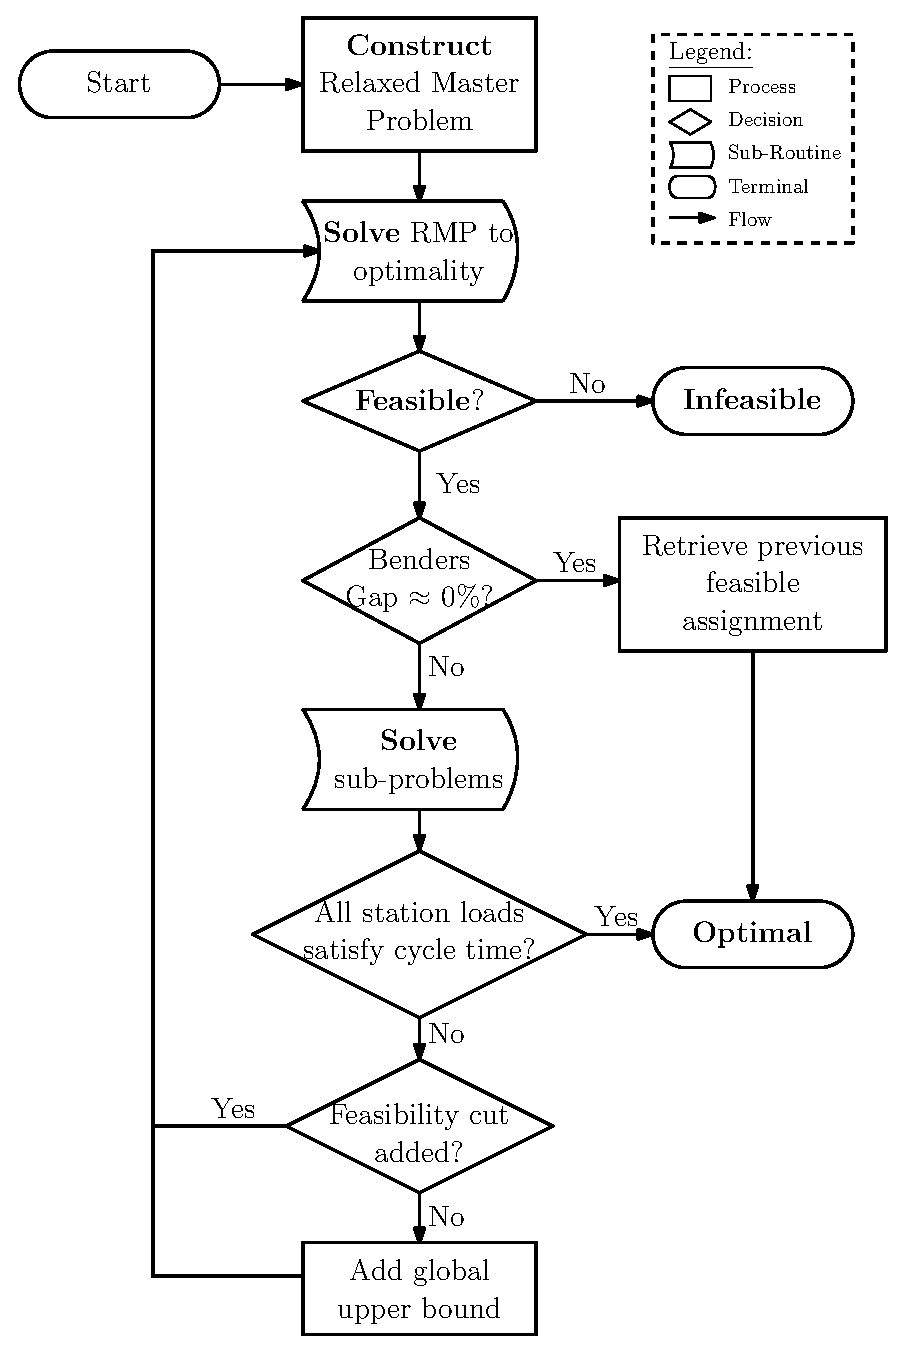
\includegraphics[height=0.95\textheight]{images/Benders-Optimality-Flowchart.eps}
	\label{fig:bend:RMPflowchart}
\end{figure}

\subsection{The Sub-Problem}
\label{sec:bend:algSP}
Once the assignment of tasks to the $m$ stations is found,
all sub-problems are solved.
Unless stated otherwise, we will only consider optimality sub-problems
for the description given here.
We now refer the reader to Figure \ref{fig:bend:SPflowchart}
for an overview of how a single sub-problem is processed.
We first check if the current assignment to the station
has been solved previously or not.
All previous solutions are stored together with their optimal station
load values, so if we find an assignment which has already been processed,
then we retrieve the previous solution and move to the next sub-problem.
In the case of a new assignment of tasks, the sub-problem
is constructed and solved to optimality.

When a sub-problem is found to be infeasible a logic cut
is added; when the load does not satisfy the current cycle time
an infer cut is added; and if the cycle time is satisfied then
no cut is generated.
In all three cases, the resulting solution is stored with
the current assignment for future referral.
The process continues on to the next sub-problem until none remain and
then returns to the master.

\begin{figure}[tbp]
	\centering
	\caption{Flowchart of an optimality sub-problem}
	\vspace{2mm}
	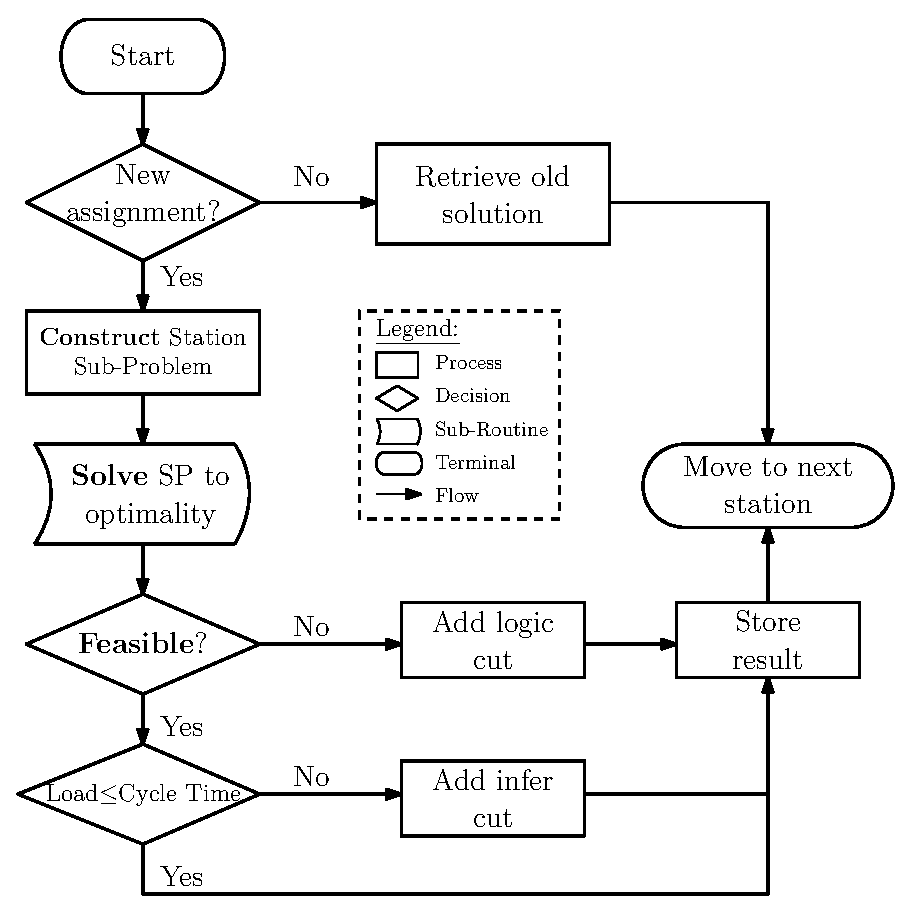
\includegraphics[width=0.95\textwidth]{images/Optimality-SP-Flowchart.eps}
	\label{fig:bend:SPflowchart}
\end{figure}

\subsection{Heuristic Approach}
We conclude this chapter by mentioning a minor modification
that can be made to the above procedure.
We only considered a tolerance of $0\%$ on the Bender
gap, however we could instead take $\varepsilon>0$.
This would result in our exact solution methodology becoming
a heuristic method able to guarantee a pre-defined
quality on the assignment and schedule found.
For example, if we set $\varepsilon=0.05$, then the
algorithm will terminate once a globally feasible solution is found
which is within $5\%$ of the optimal.
The modification of this parameter 
offers this logic-based Benders decomposition
a higher degree of flexibility.
It is possible that reaching a gap of $5\%$ can be done very efficiently
but finding the global optimal is intractable.
In practice, the industry representative
may only require feasible solutions of this quality
as the sub-optimal solution could still be superior to their 
current assembly line design.


